\section{Portfolio: The Rlaan}
Ships overview for all groups (Work In Progress): \href{http://vegastrike.sourceforge.net/wiki/Artstyle\_guide:Overview\_Guide}{Ship Overview} \\
Art-style Guide (Work In Progress): \href{http://vegastrike.sourceforge.net/wiki/Artstyle\_guide:Rlaan}{Artstyle Guide} \\
Species overview: \href{http://vegastrike.sourceforge.net/wiki/Species:Rlaan}{Species:Rlaan} \\

The artstyles for ships and installations contained in this guide applies to all the members of the Rlaan Assembly (all the subfactions, including their client races, the Lmpl, Nuhln, and the Saahasayaay). 

\subsection{Origin}
\begin{itemize}
\item Sector: 
\item System: 
\item Origin Planet:  
\item Gravity: 
\item Atmosphere: 
\item Primary liquid bodies: 
\item Average temperature of homeworld (pre-industrialization):
\item Sun: 
\item Primary challenges (pre-industrialization): 
\end{itemize}

%ORIGIN COMMENTS GO HERE

\subsubsection{Habitat}

\subsection{Physical}
\begin{itemize}
\item Dimensions: 
\item Mass: 
\item Skeletal system: 
\item Major divisions: 
\item Senses: 
\item Visual acuity: 
\item Chemosense: 
\item Locomotion: 
\item Manipulators: 
\item Textural appearance: 
\end{itemize}

%PHYSICAL COMMENTS GO HERE

\subsection{Mental}


\subsection{Technological}
\begin{itemize}
\item Tech: 
\item Weapons:
\item Tactics:
\begin{itemize}
\item    Small groups: 
\item    Large groups/Fleets: 
\end{itemize}

\item Installations:

\end{itemize}

\subsection{Culture}

\subsubsection{Factions and Organizational Groups}
Listed below are noteworthy Rlaan sub-factions and organizational groups: 
\begin{itemize}
\item FACTIONS GO HERE
\end{itemize}

\subsubsection{Religion}

\subsubsection{Cultural Aesthetics}

\subsection{Writing, numbers, and insignia}

\subsection{Faction: PRIMARY FACTION}

\subsubsection{A Brief History of the PRIMARY FACTION}


\subsubsection{Development}

\subsubsection{Culture}

\subsubsection{Organization}

\subsection{Faction: OTHER FACTIONS}

\subsection{Vessels Style}

\subsubsection{Style Overview}
\begin{itemize}

\item Primary distinguishing color ranges: 
\item Common accent colors:
\item Primary lighting color:
\item Frequently visible: 
\item Rarely visible:
\item Seen inside, but not out: 
\item Moving parts(non-turret): 
\item Capital vs. light craft: 
\end{itemize}

Rlaan ships and installations are bioengineered and are living organisms; they possess lightning fast reason-processing and reflex mechanisms though they all operate at the instinctual level (less a brain than a microchip). Although living, they contain no self-awareness and as such are supposed to be treated only as machines (in the current sense of the metaphor; as the Mechanists, the Unadorned, and the Andolians treat machines quite differently... not to mention the sentient "machines" themselves, the Unadorned Servant AI, the Mechanist Advanced AI, and the Andolian Purth) - mostly due to Rlaan expertise at creating complex instinctual neural pathways and their express lack of interest in creating sentience from nothing. Humans and pilots of other species, however, impart (erroneously) a sinister though coldly impartial personification of the Rlaan ships' minds and prefer to steer clear of piloting any of them. Nevertheless, any sentient or sub-sentient (the use of the term sub-sentient itself is debatable ;) ) being can easily pilot any of the Rlaan ships through a variety of interfaces available by specification growth.

Key Features:

A. Listed below are the basic required features of all Rlaan ships:

	1. Absence of visible incendiary means of propulsion.
	
	2. Presence of radiator/shield manipulator fins. Please take note that the fins must be 	accurate indicators of ship size. 
	
		Hence larger ships will have
		
		a) fins with a higher number of ribs (Fig.~\ref{fig:rlaan-fins}); or
		
		b) a larger number of fins, present in tiers if possible, i.e. dorsal piscine fins in 		contrast to the jutting lateral piscine fins of fighters and smaller ships.

\begin{figure}
\begin{center}
\makebox[\textwidth][c]{
    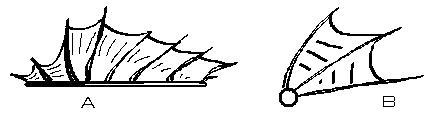
\includegraphics[width=\textwidth]{../images/styles/rlaan-fins.png}
}
    \caption{Rlaan fins with a higher number of ribs for large vessels.}
    \label{fig:rlaan-fins}
\end{center}
\end{figure}

\begin{figure} \begin{center}
	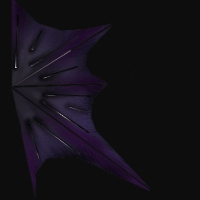
\includegraphics[width=0.4\textwidth]{../images/styles/rlaan-fins2.png}
    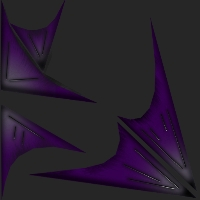
\includegraphics[width=0.4\textwidth]{../images/styles/rlaan-fins3.png}
    \caption{Samples of fin textures from in-game Rlaan ships.}
    \label{fig:rlaan-fins2}
\end{center} \end{figure}


3. Basic form is smooth and flowing, totally organic. Bilateral symmetry is a requirement 	for most of their ships. Bilateral symmetry is indicative to Rlaans of speed and agility (and 	also of 	spuriousness, contrasting their own lumbering radial symmetry - symbolic of 	precision and versatility - to the more common bilateral symmetry of other known species. 	Hence a bilaterally symmetrical vehicle is as attractive to an Rlaan as a sports car is to a 	human). Radially symmetrical ships do exist, though most are inexpensive civilian 	transports and utility ships.

4. Base Colors

5. Base Textures

	B. Listed below are the basic required features of all Rlaan installations:

	C. General Rlaan technological features (some features common in Rlaan art and architecture, devices, surface vehicles, etc.)


\subsubsection{Surface features of large vessels}

\subsubsection{Small things found on the hull of a large  vessel}
\begin{itemize}
\item Service/Maintenance hatches
\end{itemize}
{\it Somewhat larger things found on the hull of a large Aeran vessel:}
\begin{itemize}
\item Escape pod launcher ports
\end{itemize}
{\it Yet larger things ... :}
\begin{itemize}
\item Pinnace/lander launch bay (non-carrier vessels)
\end{itemize}

\subsection{Vessels Listing}

    1. Aidi(Rlaan Passenger Puddle Jumper) 
    2. Andi(Rlaan Sub-Orbital Cargo transport) 
    3. Chengdi(Rlaan Lander) 
    4. Chengzong(Rlaan Refuse and Salvage Scow) 
    5. Chongdi(Rlaan Cargo Shuttle) 
    6. Chudi(Rlaan Resupply Ship) 
    7. Daizong(Rlaan Methane Flight Tender) 
    8. Dezong(Rlaan Battleship) 
    9. Duanzong(Rlaan Orbital Sniper Ship) 
    10. Duzong(Rlaan Occupation Vessel) 
    11. Feidi(Rlaan Dropship) 
    12. Gaodi(Rlaan Forcible Compliance Planetary Drone Craft) 
    13. Gaozong(Rlaan Mobile Sensor Drone) 
    14. Gaozu(Rlaan Oxygen Flight Tender) 
    15. Gondi(Rlaan Colonization ship) 
    16. Gongti(Rlaan Oxygen client colonization ship) 
    17. Guangzong(Rlaan Repair/Maintenance craft) 
    18. Han(Rlaan Exploration Ship) 
    19. (Rlaan Constructed for non-Rlaan use) Janissary {Rlaan constructed Saahasayaay Heavy Fighter} 
    20. Shangdi(Rlaan Bulk Transport) 
    21. Shenzong(Rlaan Cargo mover) 
    22. Shizong(Rlaan Light Equalizer Ship) 
    23. Taizu(Rlaan Methane Breather Heavy Cargo Shuttle) 
    24. Wendi(Rlaan Prisoner Transport) 
    25. Wudi(Rlaan Ship Impound Transport) 
    26. Xianzong(Rlaan Mining Craft) 
    27. Xiaozong(Rlaan Patrol Corvette) 
    28. Xizong(Rlaan Oxygen Breather Heavy Cargo Shuttle) 
    29. Xuande(Rlaan Light Passenger Transport) 
    30. Xuanzong(Rlaan Gas Miner) 
    31. Yindi(Rlaan Equalizer Extermination Craft) 
    32. Zhaozong(Rlaan Heavy Equalizer Ship) 
    33. Zhezong(Rlaan Large Passenger Liner) 

\subsection{Stations Listing}

Note: For modelers wondering about the list of the Rlaan stations, there are none. Stations are not named, in the way ships are. But if you insist... ;) here's a list of the needed Rlaan installations. Don't worry, alien stations do not need to be necessarily obvious as to their functions, so if your station model looks Rlaan, it would certainly fit comfortably into any of the blank station spots. Please read guides above though for the specifics of some stations.

    1 Rlaan Medical
    2 Rlaan Factory
    3 Rlaan Research
    4 Rlaan Relay
    5 Rlaan-Briin Medical Procedure Station
    6 Rlaan-Briin Bio-mod Research
    7 Rlaan Prison Station
    8 Rlaan Repair and Salvage Station
    9 Rlaan Civilian Shipyard
    10 Rlaan Mining Base
    11 Rlaan Refinery
    12 Rlaan Military Shipyard)
    13 Rlaan Jump Point Fortifications
    14 Rlaan Weapons Platform
    15 Rlaan Anti-matter Refinery
    16 Rlaan Civilian Population Defense Redoubt
    17 Rlaan Asteroid Fighter Base
    18 Rlaan Fighter Barracks
    19 Rlaan Star Fortress


% LocalWords:  Aerans Aeran Artstyle Aera Pinnace Acrotatus Agasicles Agesilaus
% LocalWords:  Agesipolis Agis Alcmenes Anaxander Wiki Anaxandridas Rlaan Areus
% LocalWords:  Anaxidamus Ariston Charillus Cleombrotus Cleomenes Demaratus Uln
% LocalWords:  Theopompus Dorissus Echestratus Eurycratides Eurypon Leons Bzbr
% LocalWords:  Nicander Pausanias Pleistarchus UnAeranned Pleistoanax Andolian
% LocalWords:  Spaceborn's MacGyver Polydectes Polydorus EVAs Procles Prytanis
% LocalWords:  Soos Teleclus terraforming Aenethforming Zeuxidamus homeworld
% LocalWords:  coreward chemoreception Klk'k Aeneth ecologies Shmrn
